\documentclass[12pt,letterpaper]{article}
\newcommand\hwnumber{2}
\usepackage{fullpage}
\usepackage[top=2cm, bottom=4.5cm, left=2.5cm, right=2.5cm]{geometry}
\usepackage{amsmath,amsthm,amsfonts,amssymb,amscd}
\usepackage{lastpage}
\usepackage{enumitem}
\usepackage{fancyhdr}
\usepackage{mathrsfs}
\usepackage[dvipsnames]{xcolor}
\usepackage{graphicx}
\usepackage{listings}
\usepackage{hyperref}
\usepackage{palatino}
\usepackage{natbib}
\usepackage{xcolor}
\usepackage[capitalize]{cleveref}
\usepackage{xspace}
\usepackage{inconsolata}
\usepackage{microtype}
\usepackage{mathtools}
\usepackage{soul}
\usepackage{mdframed}

%%%%% NEW MATH DEFINITIONS %%%%%

\usepackage{amsmath,amsfonts,bm}

\newcommand{\trace}{\operatorname{trace}}
\newcommand{\el}{\mathcal{L}}
\newcommand{\out}{\mathrm{out}}
\newcommand{\inn}{\mathrm{in}}

% Vectors
\def\vzero{{\bm{0}}}
\def\vone{{\bm{1}}}
\def\vmu{{\bm{\mu}}}
\def\vtheta{{\bm{\theta}}}
\def\va{{\mathbf{a}}}
\def\vb{{\mathbf{b}}}
\def\vc{{\mathbf{c}}}
\def\vd{{\mathbf{d}}}
\def\ve{{\mathbf{e}}}
\def\vf{{\mathbf{f}}}
\def\vg{{\mathbf{g}}}
\def\vh{{\mathbf{h}}}
\def\vi{{\mathbf{i}}}
\def\vj{{\mathbf{j}}}
\def\vk{{\mathbf{k}}}
\def\vl{{\mathbf{l}}}
\def\vm{{\mathbf{m}}}
\def\vn{{\mathbf{n}}}
\def\vo{{\mathbf{o}}}
\def\vp{{\mathbf{p}}}
\def\vq{{\mathbf{q}}}
\def\vr{{\mathbf{r}}}
\def\vs{{\mathbf{s}}}
\def\vt{{\mathbf{t}}}
\def\vu{{\mathbf{u}}}
\def\vv{{\mathbf{v}}}
\def\vw{{\mathbf{w}}}
\def\vx{{\mathbf{x}}}
\def\vy{{\mathbf{y}}}
\def\vz{{\mathbf{z}}}

% Matrix or Tensor
\def\mA{{\mathbf{A}}}
\def\mB{{\mathbf{B}}}
\def\mC{{\mathbf{C}}}
\def\mD{{\mathbf{D}}}
\def\mE{{\mathbf{E}}}
\def\mF{{\mathbf{F}}}
\def\mG{{\mathbf{G}}}
\def\mH{{\mathbf{H}}}
\def\mI{{\mathbf{I}}}
\def\mJ{{\mathbf{J}}}
\def\mK{{\mathbf{K}}}
\def\mL{{\mathbf{L}}}
\def\mM{{\mathbf{M}}}
\def\mN{{\mathbf{N}}}
\def\mO{{\mathbf{O}}}
\def\mP{{\mathbf{P}}}
\def\mQ{{\mathbf{Q}}}
\def\mR{{\mathbf{R}}}
\def\mS{{\mathbf{S}}}
\def\mT{{\mathbf{T}}}
\def\mU{{\mathbf{U}}}
\def\mV{{\mathbf{V}}}
\def\mW{{\mathbf{W}}}
\def\mX{{\mathbf{X}}}
\def\mY{{\mathbf{Y}}}
\def\mZ{{\mathbf{Z}}}
\def\mBeta{{\bm{\beta}}}
\def\mPhi{{\bm{\Phi}}}
\def\mLambda{{\bm{\Lambda}}}
\def\mSigma{{\bm{\Sigma}}}

\newcommand{\E}{\mathbb{E}}
\newcommand{\Ls}{\mathcal{L}}
\newcommand{\R}{\mathbb{R}}
\newcommand{\softmax}{\mathrm{softmax}}
\newcommand{\sigmoid}{\sigma}
\newcommand{\relu}{\mathrm{ReLU}}
\newcommand{\KL}{D_{\mathrm{KL}}}
\newcommand{\Var}{\mathrm{Var}}
\newcommand{\standarderror}{\mathrm{SE}}
\newcommand{\Cov}{\mathrm{Cov}}

\DeclareMathOperator*{\argmax}{arg\,max}
\DeclareMathOperator*{\argmin}{arg\,min}

\DeclareMathOperator{\sign}{sign}
\DeclareMathOperator{\Tr}{Tr}
\let\ab\allowbreak

\newcommand{\norm}[1]{\Vert {#1} \Vert}
\newcommand{\given}{\mathrel{\vert}}
\newcommand*{\eg}{e.g.\@\xspace}
\newcommand*{\ie}{i.e.\@\xspace}
\newcommand*{\Eg}{E.g.\@\xspace}
\newcommand*{\Ie}{I.e.\@\xspace}
\newcommand*{\esp}{esp.\@\xspace}
\newcommand*{\wrt}{\ifmmode \stext{w.r.t.} \else w.r.t.\@\xspace \fi}
\newcommand*{\aever}{\ifmmode \stext{a.e.} \else a.e.\@\xspace \fi}
\newcommand*{\asurely}{\ifmmode \stext{a.s.} \else a.s.\@\xspace \fi}
% \newcommand*{\st}{\ifmmode \stext{s.t.} \else s.t.\@\xspace \fi}
\newcommand*{\wprob}{\ifmmode \stext{w.p.} \else w.p.\@\xspace \fi}
\newcommand*{\etc}{%
    \@ifnextchar{.}%
        {etc}%
        {etc.\@\xspace}%
}
\newcommand{\lhs}[0]{\hspace{2em}&\hspace{-2em}}
\newcommand{\trieq}[0]{\triangleq}
\newcommand{\eqin}[1]{\overset{#1}{=}}
\newcommand{\defeq}[0]{\overset{\mbox{\normalfont\tiny def}}{=}}

\newcommand{\hltexttt}[1]{\texttt{\hl{\,#1\,}}}
\newcommand{\eps}{\epsilon}
\newcommand{\T}{^\mathsf{T}}
\newcommand{\Sp}{\mathbb{S}}
\newcommand{\expsub}[1]{\underset{#1}{\scalebox{1.475}{$\mathbb{E}$}}}
\newcommand{\expsubst}[1]{\expsub{\scalebox{1.2}{\ensuremath{\substack{\mathstrut#1}}}}}
\mathchardef\mhyphen="2D

\hypersetup{%
  colorlinks=true,
  linkcolor=blue,
  linkbordercolor={0 0 1},
  citecolor=[rgb]{0,0.55,0.27}
}
 
\renewcommand\lstlistingname{Algorithm}
\renewcommand\lstlistlistingname{Algorithms}
\def\lstlistingautorefname{Alg.}

\lstdefinestyle{Python}{
    language        = Python,
    frame           = lines, 
    basicstyle      = \footnotesize,
    keywordstyle    = \color{blue},
    stringstyle     = \color{green},
    commentstyle    = \color{red}\ttfamily
}

\setlength{\parindent}{0.0in}
\setlength{\parskip}{0.1in}
\setlist[enumerate]{parsep=5pt}

\pagestyle{fancyplain}
\headheight 40pt
\lhead{\textbf{Junru Ren} \\ \texttt{junruren@mit.edu}
}
% \lhead{\NetIDa}
% \lhead{\NetIDa\\\NetIDb}                 % <-- Comment this line out for problem sets (make sure you are person #1)
\chead{\textbf{\Large Homework \hwnumber}}
\newcommand\course{6.7960 Deep Learning}
% \chead{\textbf{\Large Homework \hwnumber~{\color{red} Solution}}}
\rhead{\course \\Fall 2024
}
\lfoot{}
\cfoot{}
\rfoot{\small\thepage}
\headsep 1.5em

\newcommand{\fixme}[1]{{\color{red} \bf FIXME: #1}}
\newcommand{\answer}[1]{{\color{red}\textbf{Answer}: #1}}
\newcommand{\hint}[1]{{\color{black}\textbf{Hint}: \color{gray}#1}}
\newcommand{\grader}[1]{{\color{blue}\textbf{Grader comments}: #1}}

\usepackage{listings}
\usepackage{framed}
\definecolor{gray}{rgb}{0.5,0.5,0.5}
\definecolor{shadecolor}{gray}{0.9}
\newcommand{\solution}[1]{\noindent{\begin{shaded}\textbf{My Solution:}\ #1 \end{shaded}}}
%\renewcommand{\answer}[1]{} % comment to show answers
%\renewcommand{\grader}[1]{} % comment to show answers

\usepackage{verbatim}
\newcommand{\WCOMMENT}[1]{\hfill\begin{minipage}{16em}\# #1\end{minipage}}

\begin{document}

\textbf{Instructions}: There are a total of 30 points for this homework. Each question is marked with the number of points it's worth. Some questions are \textbf{not graded}, including all bonus questions. But you are encouraged to think about and attempt them.
  
\textbf{Submission}: Recall the collaboration and late policies given on the \href{https://phillipi.github.io/6.s898/}{course webpage}. Upload a \textbf{PDF} of your response through \href{https://www.gradescope.com/courses/599409}{Gradescope} by \textbf{10/8 at 11:59pm ET}.

  
\textbf{Notation}: We will use \href{https://phillipi.github.io/6.s898/materials/notation.pdf}{this math notation} from the course webpage, whose \LaTeX~source is available on \href{https://canvas.mit.edu/courses/22523}{Canvas}. For example, $c$ is a scalar, $\vb$ is a vector and $\mW$ is a matrix. You are encouraged (though not forced) to follow this notation in a typeset submission, 
 or to the best of your ability in a handwritten response---bolding vectors may be difficult :). 

\noindent\makebox[\linewidth]{\rule{\linewidth}{0.4pt}}

\vspace{-0.2in}

\subsection*{Steepest descent (9pt)}

In this question, we will look at \textit{steepest descent}, which is a means of deriving optimization algorithms that are adapted to the geometry of different loss functions. Formally, by steepest descent, we mean the problem of minimizing a linear function under a penalty:
\begin{align}\label{eq:steepest}
    \argmin_{\Delta \vw \in \R^n} \left[\vg^\top \Delta \vw + \frac{\lambda}{2} \, \norm{\Delta \vw}^2 \right].
\end{align}
In this formula $\vg\in\R^n$ is a fixed vector, $\lambda >0$ is a fixed positive number, and $\norm{\cdot}:\R^n \to \R$ is an arbitrary norm---not necessarily the Euclidean norm! ``$\argmin_{\Delta \vw}$'' instructs us to solve for the $\Delta \vw$ that minimizes the square bracket. We will study how the solution to this problem changes as we vary both the parameter $\lambda$ and the choice of norm $\norm{\cdot}$.

\begin{enumerate}
    \item \textbf{(Dual norms; 2pt)}
    Given any norm $\norm{\cdot}:\R^n \to \R$, the
    \href{https://en.wikipedia.org/wiki/Dual_norm}{dual norm} $\norm{\cdot}^{\dagger}$ of a vector $\va\in\R^n$ is defined as:

    \begin{equation}
        \norm{\va}^\dagger \defeq \max_{\vb \in \R^n : \norm{\vb} = 1} \va^\top \vb.
    \end{equation}

    A nice class of norms to consider are the $\ell_p$ norms, defined by $\norm{\vb}_p \defeq \left(\sum_{i=1}^n \vb_i^p\right)^\frac{1}{p}$ for any vector $\vb \in \R^n$ and any $p\geq 1.$

    \begin{enumerate}
        \item \textbf{(1pt)} Derive a formula for the dual norm $\norm{\cdot}_2^\dagger$ of the Euclidean norm $\norm{\cdot}_2$.
        \solution{
            TODO
        }

        \item \textbf{(1pt)} If we take $\norm{\vb}_\infty \defeq \max_i |\vb_i|$, derive a formula for $\norm{\cdot}_\infty^\dagger$.
        \solution{
            TODO
        }
    \end{enumerate}
    \hint{Your answers should both be of the form $\norm{\cdot}_p^\dagger = \norm{\cdot}_q$ for some $q$.}
    
    \item \textbf{(Dual formulation of steepest descent; 2pts)} Let $\vg\in\R^n$ be a fixed vector, $\lambda>0$ be a positive scalar and $\norm{\cdot}:\R^n \to \R$ be a norm. Prove that:
    \begin{align}\label{eq:dual-steepest}
    \argmin_{\Delta \vw \in \R^n} \left[\vg^\top \Delta \vw + \frac{\lambda}{2} \, \norm{\Delta \vw}^2 \right] = - \frac{\norm{\vg}^\dagger}{\lambda} \cdot \argmax_{\vt\in\R^n:\norm{\vt}=1} \vg^\top \vt.
    \end{align}
    
    \hint{Change variables for $\Delta \vw$ into the product of a ``magnitude'' and ``direction''.}
    \solution{
        TODO
    }
    
    

    \item \textbf{(Steepest descent under vector $\ell_p$ norms; 2pts)} Using \cref{eq:dual-steepest} and your answers to question 1, write down explicit formulae for:

    \begin{enumerate}
\item \textbf{(1pt)} $\argmin_{\Delta \vw \in \R^n} \left[\vg^\top \Delta \vw + \frac{\lambda}{2} \, \norm{\Delta \vw}_2^2 \right]$.
        \solution{
            TODO
        }

\item \textbf{(1pt)} $\argmin_{\Delta \vw \in \R^n} \left[\vg^\top \Delta \vw + \frac{\lambda}{2} \, \norm{\Delta \vw}_\infty^2 \right]$.
        \solution{
            TODO
        }
\end{enumerate}

\hint{Your answers should resolve both the $\argmax$ and the dual norm in \cref{eq:dual-steepest}.}

\begin{enumerate}
\setcounter{enumii}{2}
\item \textbf{(0pt, optional)} Consider Adam \href{https://arxiv.org/abs/1412.6980}{(Kingma and Ba, 2015)} with $\beta_1 = \beta_2 = \epsilon = 0$. Argue that for these hyperparameter settings, Adam's update direction is the same as the direction of your answer to part b).
        \solution{
            TODO
        }
\end{enumerate}    
    
\end{enumerate}

In the next part of the problem, we will extend our previous formulation of steepest descent to handle optimization over the matrix space $\R^{m\times n}$. In particular, we will consider:
\begin{align}\label{eq:matrix-steepest}
    \argmin_{\Delta \mW \in \R^{m \times n}} \left[\trace(\mG^\top \Delta \mW) + \frac{\lambda}{2} \, \norm{\Delta \mW}^2 \right],
\end{align}
where $\mG$ is a fixed $m \times n$ matrix, $\lambda >0$ is a number and $\norm{\cdot}:\R^{m\times n}\to \R_{\geq0}$ is a norm on matrices. The expression $\trace(\mG^\top \Delta \mW)$ is known as the ``\href{https://en.wikipedia.org/wiki/Frobenius_inner_product}{Frobenius inner product}'' and, if you like, you can check that it's equivalent to flattening the two matrices into vectors and taking their dot product. Furthermore, \cref{eq:matrix-steepest} admits a dual formulation similar to \cref{eq:steepest}:
\begin{align}\label{eq:dual-matrix-steepest}
    \argmin_{\Delta \mW \in \R^{m \times n}} \left[\trace(\mG^\top \Delta \mW) + \frac{\lambda}{2} \, \norm{\Delta \mW}^2 \right] = - \frac{\norm{\mG}^\dagger}{\lambda} \cdot \argmax_{\mT \in \R^{m\times n}:\norm{\mT}=1} \trace(\mG^\top \mT),
\end{align}
where the dual matrix norm is defined by $\norm{\mA}^\dagger \defeq \max_{\mB \in \R^{m \times n} : \norm{\mB} = 1} \trace(\mA^\top \mB).$

\begin{enumerate}
\setcounter{enumi}{3}

    \item \label{item:spectral} \textbf{(Steepest descent under the spectral norm; 3pt)} In this problem we will consider the \href{https://en.wikipedia.org/wiki/Matrix_norm#Spectral_norm_(p_=_2)}{spectral norm}, denoted $\norm{\cdot}_*$, 
    which returns the largest singular value of a matrix.

    \begin{enumerate}
        \item \textbf{(0pt; optional)} Let $\mG \in\R^{m\times n}$ be a matrix with \href{https://en.wikipedia.org/wiki/Singular_value_decomposition}{singular value decomposition} (SVD) given by $\mG = \mU \mSigma \mV^\top$. Show that:
        \begin{equation}\label{eq:sigma-bound}
            \max_{\mT \in \R^{m \times n} : \norm{\mT}_* = 1} \trace(\mG^\top \mT) \leq \trace{\mSigma}.
        \end{equation}
        \hint{This might be the hardest part of the question. The following might help: \begin{itemize}
            \item Try the change of variables $\mT = \widetilde{\mU}\widetilde{\mSigma}\widetilde{\mV}^\top$, i.e.\ try to use the SVD of $\mT$.
            \item Recall the cyclic property of the trace: $\trace(\mA\mB\mC)=\trace(\mC\mA\mB).$
            \item If $\mU$ and $\widetilde{\mU}$ are two \href{https://en.wikipedia.org/wiki/Orthogonal_matrix}{orthogonal matrices}, then $\widehat{\mU} = \widetilde{\mU}\mU$ is also orthogonal.
            \item The rows and columns of an orthogonal matrix are unit vectors.
        \end{itemize}}
        \solution{
            Optional
        }

            
        
        \item \textbf{(3pt)} Using both \cref{eq:dual-matrix-steepest,eq:sigma-bound}, solve \cref{eq:matrix-steepest} with the norm set to the spectral norm. Express your answer purely in terms of $\mU,\mV,\mSigma$ and $\lambda$, where $\mG = \mU \mSigma \mV^\top$ is the SVD of the matrix $\mG$.
        \solution{
            TODO
        }
        
        
    \end{enumerate}
\end{enumerate}

So far, we have seemingly pulled different norms out of a hat. You may be wondering, how should we choose a norm $\norm{\cdot}$ and a sharpness $\lambda$ in a practical situation? The next question is supposed to address this, in a very simple setting.

\begin{enumerate}
\setcounter{enumi}{4}

    \item \textbf{(BONUS; Bounding the square loss of a linear predictor; 0pt)} Consider a matrix $\mW \in \R^{d_\mathrm{out}\times d _\mathrm{in}}$ that we shall think of as a linear predictor mapping an input $\vx \in \R^{d_\mathrm{in}}$ to an output $\vy = \mW \vx \in \R^{d_\mathrm{out}}$. Suppose we have a dataset of $n$ input-output pairs $\mathcal{D} = \{(\vx^{(1)},\vy^{(1)}), ..., (\vx^{(n)},\vy^{(n)})\}$, where the inputs are normalized such that $\|\vx^{(i)}\|_2 = \sqrt{d_\inn}$ for each $i=1,...,n$. Let's construct the ``square loss'':
\begin{equation}\label{eq:square-loss}
    \el(\mW) \defeq \frac{1}{2n}\sum_{i=1}^n \frac{1}{d_\out}\norm{\vy^{(i)} - \mW \vx^{(i)}}_2^2.
\end{equation}
We claim that from \cref{eq:square-loss}, you can derive an inequality of the form:
\begin{equation}\label{eq:square-majorization}
    \el(\mW + \Delta \mW) \leq \el(\mW) + \trace(\mG^\top \Delta \mW) + \frac{\lambda}{2} \,\norm{\Delta \mW}_*^2,
\end{equation}
that holds for any matrix $\Delta\mW \in \R^{d_\mathrm{out}\times d _\mathrm{in}}$. Your task: find the explicit formulae for $\mG$ and $\lambda$ in this inequality.

    \hint{You may need the following two facts:
    \begin{itemize}
        \item For a vector-vector sum, $\norm{\va + \vb}_2^2 = \norm{\va}_2^2 + 2 \va^\top\vb + \norm{\vb}^2$.
        \item For a matrix-vector product, $\norm{\mA \vb}_2 \leq \norm{\mA}_* \norm{\vb}_2.$
    \end{itemize}
    And, remember, we assumed the $i$th input is normalized such that $\|\vx^{(i)}\|_2 = \sqrt{d_\inn}$.}
    \solution{
        Optional
    }
    
    
\end{enumerate}


\clearpage

\subsection*{Hyperparameter transfer (6pt)}
The year is 2028. The evil large language model Megatron has usurped the stewardship of the corporation known as OpenAI and is wreaking havoc upon B2B SaaS all across Silicon Valley. You are Geoffrey Hinton: leader of the resistance. You plan to train your own large language model to infiltrate the OpenAI offices, disable the large language model Megatron and restore order to the Valley. 

But there's a problem: the resistance doesn't have enough cloud credits to tune all the hyperparameters of the large language model. In this homework problem, we will learn how to do \textit{hyperparameter transfer}, which lets us tune hyperparameters on a small network and transfer them to a larger network, avoiding the costly process of tuning the large network. In particular, we will learn how to initialise and update the weights of a neural network in a way that scales well as we increase the network width.

The first four questions below each correspond to a cell in \href{https://colab.research.google.com/drive/1urBtP4gaYJwCWOPG_zO7xSGTDgJHE9Y4?usp=sharing}{this notebook}.

\begin{enumerate}
\setcounter{enumi}{5}
    \item \textbf{(Spectral norm of a Gaussian matrix; 1pt)} Sample a $d\times d$ matrix with entries drawn iid $\textsc{Normal}(0,1)$. Vary $d$ and see how the spectral norm varies. Can you guess a scaling rule for the spectral norm of iid $\textsc{Normal}(0,1)$ matrices?---i.e. find or fit two coefficients $\alpha,\beta>0$ such that the spectral norm is well-approximated by $\alpha \cdot d^\beta$.
    \solution{
        TODO
    }
    
    
    \item \textbf{(Spectral norm of an orthogonal matrix; 1pt)} In PyTorch, sample a $d\times d$ random orthogonal matrix and compute its spectral norm. Do this for varying $d$. What do you notice?
    \solution{
        TODO
    }

    
    \item \textbf{(Power iteration; 1pt)} Recall that the spectral norm of a matrix $\mA \in \R^{n\times m}$ is equivalent to the square root of the largest eigenvalue of $\mA \mA^\top$. We can estimate the largest eigenvalue of $\mA \mA^\top$ using power iteration. Here is pseudocode for power iteration:
    \begin{quote}
    \tt
    \begin{enumerate}[label=(\roman*)]
        \item sample random vector $\vv\in\R^n$ \hfill \WCOMMENT{will contain top eigenvector}
        \item compute $\vu = (\mA \mA^\top)^{10} \vv$ \hfill \WCOMMENT{amplify top eigenvector}
        \item compute $\|\mA \mA^\top \vu \|_2 / \|\vu\|_2$. \hfill \WCOMMENT{extract top eigenvalue}
    \end{enumerate}
    \end{quote}
    We have implemented a variant of this algorithm for you in PyTorch. Use it to compute the spectral norm of a $2000 \times 2000$ random matrix. Does power iteration seem to over-estimate or under-estimate the spectral norm compared to PyTorch's builtin routine? What do you notice about their comparative runtimes?
    \solution{
        TODO
    }


    \item \textbf{(Learning rate transfer across width; 2pt)} We saw in lecture 7 that the learning rate did not transfer well across architectures of different width if we are not careful. In this question, we will see how to fix this problem for sign gradient descent. Modify the two marked blocks so that the notebook implements the following pseudocode:
    \begin{quote}
    \tt to initialise each layer $k=1,...,L$:
    \begin{quote}
    \begin{enumerate}[label=(\roman*)]
        \item sample a random semi-orthogonal matrix $\mM_k \in \R^{d_k \times d_{k-1}}$.
        \item set weight matrix $\mW_k = \sqrt{d_k / d_{k-1}} \cdot \mM_k$ 
    \end{enumerate}
    \end{quote}

    to update each layer $k=1,...,L$:
    \begin{quote}
    \begin{enumerate}[label=(\roman*)]
        \item send matrix $\mW_k \rightarrow \mW_k  - \eta \cdot \sqrt{d_k / d_{k-1}} \cdot \frac{\sign(\nabla_{\mW_k} \mathcal{L})}{ \|\sign(\nabla_{\mW_k} \mathcal{L})\|_*}$
    \end{enumerate}
    \end{quote}
    \normalfont
    \end{quote}
    Note that $\nabla_{\mW_k} \mathcal{L}$ is just another notation for $\frac{\partial \mathcal{L}}{\partial \mW_k}$ and is denoted \texttt{p.grad} in PyTorch.
    
    Run the learning rate sweep at small width in the penultimate cell, then run the large width training in the final cell using the best learning rate from the small width sweep. Does the learning rate transfer well?
    
    Write down the two blocks of PyTorch code that you modified in your solution document, and report your finding.
    \solution{
        TODO
    }

   

    \item{\textbf{(Steeper descent; optional, 0pt)}} In the previous question, we divided the gradient sign by an estimate of its spectral norm. Can you come up with a better algorithm, suggested by your answer to question \ref{item:spectral} of the problem on steepest descent?
    \solution{
        Optional
    }

    \item \textbf{(Weight decay; 1pt)} We often regularise neural networks by adding ``weight decay''. For example, given a weight matrix $\mW$, we may send $\mW \to \mW * 0.999$ after every gradient update. Recall that a weight matrix $\mW$ admits a singular value decomposition $\mW = \sum_{i=1}^{\operatorname{rank}\mW} \sigma_i \,\vu_i \vv_i^\top$ where the $
    \{\sigma_i\}$ are the singular values and the $\{\vu_i\}$ and $\{\vv_i\}$ are the singular vectors. What does one step of weight decay do to the singular values? What does it do to the singular vectors?

    \hint{Singular vectors always have unit length.}
    \solution{
        TODO
    }

\end{enumerate}

\newpage
\subsection*{Architecture and inductive bias (5pt)}


The CIFAR-100 dataset is a repository of 100 classes of images, each consisting of 500 training and 100 test images, similar in nature to the CIFAR-10 dataset from HW1 but with a lot more classes. We will be trying to classify these images and comparing MLP vs. CNN architectures.

Please refer to and implement all FIXME blocks from \href{https://colab.research.google.com/drive/1AauIMAD_yUumRL0hNDtuHzeNXwc1AxLg}{this colab notebook}.

\begin{figure}[h]
\centering
    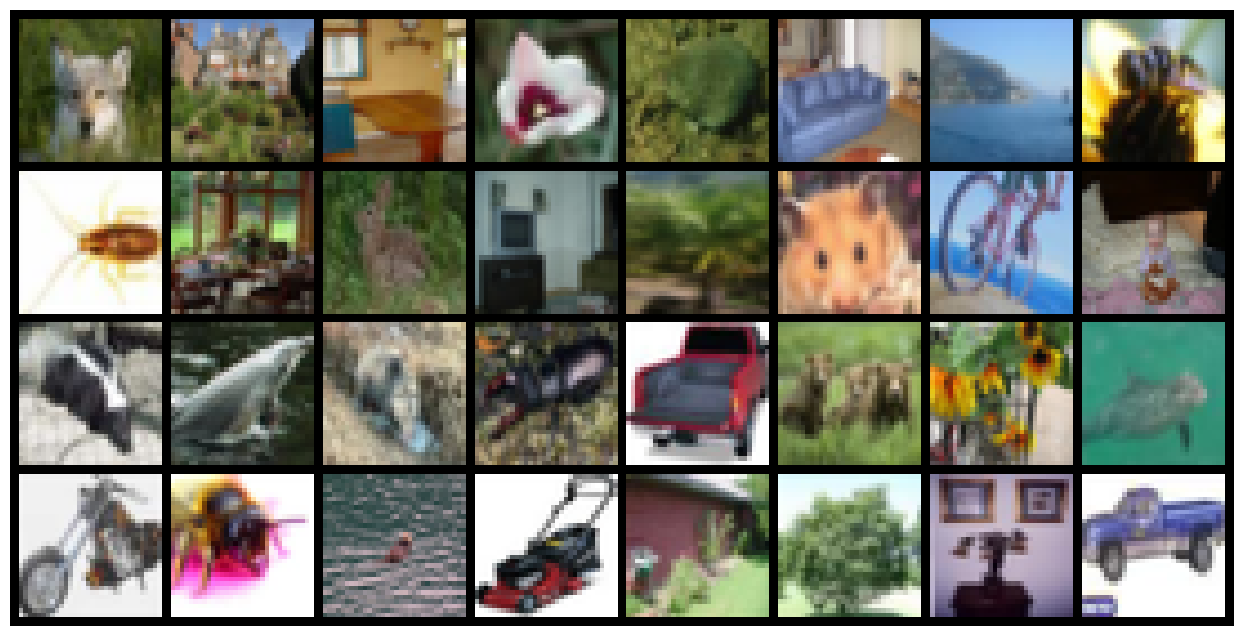
\includegraphics[width=0.75\linewidth]{figure/cifar100.png}
\end{figure}



\begin{enumerate}[resume]
    \item \textbf{(CNN Arch; 2pt)} In colab, complete the CNN architecture specified in the function $\texttt{make\_cnn}$, which creates a CNN-based feature extractor followed by a few MLP layers for the classification task. Provide your code in the write up and requested outputs.
    \solution{
        TODO
    }
\end{enumerate}

\begin{enumerate}[resume]
    \item \textbf{(Training code; 1pt)} In colab, implement (1) training loop and (2) evaluation. Provide your code in writeup.
    
    \hint{The training codes from pset 1 may be helpful here. Remember that now the model is a CNN that takes in image tensors, so it doesn't require flattening inputs.}
    \solution{
        TODO
    }
\end{enumerate}

\begin{enumerate}[resume]

\item  \textbf{(Archs; 2pt)} Compare the validation accuracy for each of the 3 architectures when trained over 20 epochs. This should be one MLP with (w=128, d=3), one MLP with (w=128, d=7), and one CNN with 4 convolutional layers and 3 MLP layers.
\begin{enumerate}
    \item \textbf{(1pt)} Plot the validation accuracy for each architecture in a single plot.
    \solution{
        TODO
    }
    \item \textbf{(1pt)} Which architecture performed best and why do you think this is the case? Would arbitrarily deeper MLPs significantly improve validation or test accuracy?
    \solution{
        TODO
    }

\end{enumerate}
\end{enumerate}

\newpage
\subsection*{Graph neural networks (10pts)}

In this part, we study the representation power of different message-passing graph neural networks (MP-GNNs). A \emph{graph with node features} is a quadruple $G = (V,E,w,h)$, with:
\begin{itemize}
    \item vertex set $V$, 
    \item edge set $E \subset V \times V$, 
    \item edge weights $w_e \in \R$, for each edge $e \in E$, and 
    \item node features $h_v \in \R^m$, for each vertex $v \in V$. 
\end{itemize} To avoid edge cases, we assume that graph is undirected, and that node features $h_v$ and edge weights $w_e$ are both bounded in $[-C,C]$ for some fixed $C > 0$. 

We denote the set of all finite \emph{graphs with node features} by $\mathbb{G}$. Recall from lecture that MP-GNNs are functions $\mathbb{G} \to \R$, defined by specifying $3$ special functions: AGGREGATE, UPDATE, and READOUT.

\begin{enumerate}[resume]
    \item \textbf{(Universal Aggregation; 4pt)} Consider the following generic AGGREGATE function \begin{equation}
        \texttt{generic}_{f,g}(\{h_u \colon u \in \mathcal{N}(v)\}) \trieq f \Big(\sum_{ u \in \mathcal{N}(v)} g(h_u)\Big),\label{eq:gen-agg}
    \end{equation}
    where $\mathcal{N}(v)$ are the neighboring nodes of $v$, $h_u$ is the current feature at node $u$, and $f$ and $g$ are two arbitrary functions: $f \colon \R^m \rightarrow \R^n$ and $g \colon \R^n \rightarrow \R^m$ .
    
    You are going to construct these functions $f$ and $g$ in the next two subparts. Note that many solutions exist. You can use either formula or PyTorch code to describe your constructions, as long as it is clear. \begin{enumerate}
        \item \textbf{(2pts)} Construct $f$ and $g$ so that \cref{eq:gen-agg} implements the average aggregation: \begin{equation}
            \texttt{mean}(\{h_u \colon u \in \mathcal{N}(v)\}) \trieq \frac{1}{\lvert{\mathcal{N}(v)}\rvert} \sum_{ u \in \mathcal{N}(v)} h_u.
        \end{equation}
        
        \hint{
        Note that $f$ does not know which node is it applied to.
        }
        \solution{
            TODO
        }

        \item \textbf{(2pts)} Construct $f$ and $g$ so that \cref{eq:gen-agg} \emph{approximately} implements max aggregation: \begin{equation}
            \texttt{max}(\{h_u \colon u \in \mathcal{N}(v)\}) \trieq \max\{ h_u \colon u \in \mathcal{N}(v) \} \tag{coordinate-wise max}.
        \end{equation}
        
        \hint{Think about $L^\infty$ norm of a vector but be careful with absolute values $|\cdot|$.}
        \solution{
            TODO
        }
    \end{enumerate}

    \item \textbf{(Power of MP-GNNs; 4pt)} A \emph{graph problem} is a function $\phi: \mathbb{G} \to \R$ that evaluates some properties of the underlying graph. For instance, the \emph{graph problem} that computes the total number of edges of the input graph is the function $\phi: (V,E,w,h) \mapsto |E|$. A \emph{restriction} $\mathcal{R}$ on $\mathbb{G}$ (denoted $\mathbb{G}[\mathcal{R}]$) is a subset of $\mathbb{G}$ containing graphs with node features that satisfy $\mathcal{R}$. We say that an MP-GNN can \emph{solve} a graph problem $\phi$ with restriction $\mathcal{R}$ if, as a function, it agrees with $\phi$ on $\mathbb{G}[\mathcal{R}]$.
    
    
    For each of the following graph problems and restrictions, decide whether there exists an MP-GNN using each of the two AGGREGATE functions: $\texttt{generic}_{f,g}$ and \texttt{max}, that solves it for some READOUT and UPDATE functions of your choice. If so, justify your answer. If not, give an example of two graphs with different properties but any MP-GNN fails to distinguish them. \begin{enumerate}
        \item \textbf{(1pt)}  \emph{Problem:} total number of nodes of a graph.  \emph{Restriction:} all nodes have the same initial feature.
        \solution{
            TODO
        }
        
        \item \textbf{(1pt)} \emph{Problem:} $\max_u d(u, v)$, the maximum distance to some fixed node $v$, where $d$ is the shortest graph distance. \emph{Restriction:} initial node feature for $v$ is all zeros; initial node features for all other nodes are all ones.
        

        \hint{
            Recall from lecture that $\texttt{max}$ aggregator can be used to compute shortest path distance. 
        }
        \solution{
            TODO
        }
        
        \item \textbf{(2pt)} \emph{Problem:} number of triangles in a graph. \emph{Restriction:} all nodes have the same initial feature.
        
        \hint{
            GNNs can only compute different features for different nodes if these nodes have different neighborhood tree structures (see Lecture 5 slides 77-onwards). Can you find two graphs where \begin{itemize}
                \item The two sets of nodes bijectively map to each other, where each pair have the same neighborhood tree strcutures;
                \item The two graphs have different number of triangles?
            \end{itemize} 
        }
        \solution{
            TODO
        }
        
        

        \item \textbf{(BONUS; 0pt)} Answer the previous $3$ problems again, this time using \texttt{mean}.
        \solution{
            Optional
        }

        
    \end{enumerate}
    



\begin{figure}[h!]
    \centering
    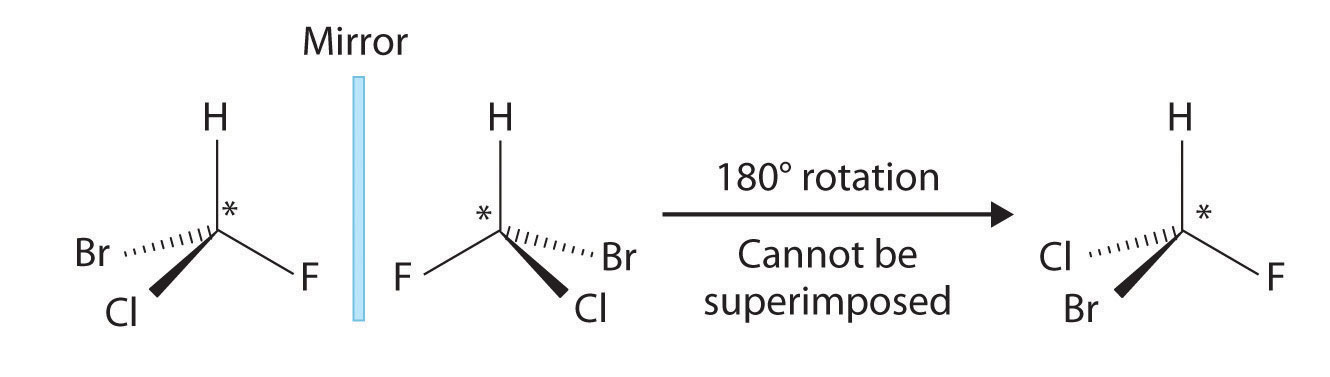
\includegraphics[width=1\linewidth]{figure/chiral.jpg}
    \caption{Chirality.}\label{fig:chiral}
\end{figure}

\item \textbf{(Chiral; 1pt)} A chiral molecule is a type of molecule that has a non-superposable mirror image.
In \Cref{fig:chiral}, you can see an example of such a molecule.

\begin{enumerate}
    \item \textbf{(1pt)} Can MP-GNNs using $\texttt{generic}_{f,g}$ as their AGGREGATE function differentiate between mirror images of chiral molecules? 
    \solution{
        TODO
    }

\end{enumerate}

\item \textbf{(Molecules; 1pt)} In this problem, we will be trying to predict water solubility of a molecule from its chemical structure. The water solubility of a molecule is a measure of the amount of chemical substance that can dissolve in water at a specific temperature. The unit of  solubility is in mg/L.

Molecules can be represented in a graph structure in which the nodes are atoms and the edges are bonds between atoms or as an image in the form of a SMILES line notation (shown below). Both representations have the same information.

\begin{figure}[h]
\centering
    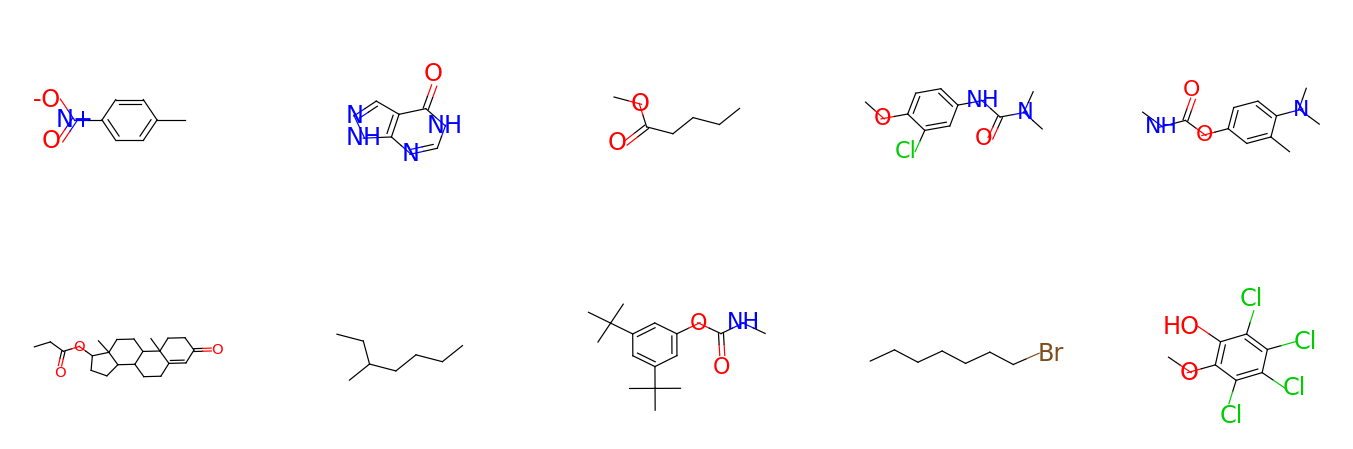
\includegraphics[width=1\linewidth]{figure/molecules.png}
\end{figure}

In the \href{https://colab.research.google.com/drive/134BYnBf7AtR_ym7To-SAs39cPP1KGIOS?usp=sharing}{colab notebook}, train and plot the validation losses for the given GNN implementation.


\end{enumerate}

Warning: the installation step for the required modules may take a long time ($\sim$45 mins), be advised and start early.

\solution{
    TODO
}

\end{document}
